% Clean AI-assisted research revision, 20 October 2026.
% The preserved supervisor source is paper_history/supervisor_draft.tex.
% Author metadata and declarations need human approval before submission.
\documentclass[5p,times,twocolumn]{elsarticle}
\usepackage[T1]{fontenc}
\input{glyphtounicode}
\pdfgentounicode=1
\usepackage{graphicx,multirow}
\usepackage{amsmath,amssymb,amsfonts,amsthm}
\usepackage{xcolor,textcomp,booktabs,tabularx,array,adjustbox}
\usepackage{placeins,dblfloatfix,listings,enumitem,url}
\usepackage{needspace}
\usepackage[hidelinks]{hyperref}
\setlength{\emergencystretch}{2em}
\Urlmuskip=0mu plus 1mu
\newcolumntype{Y}{>{\raggedright\arraybackslash\hspace{0pt}}X}
\newcolumntype{R}{>{\raggedleft\arraybackslash\hspace{0pt}}X}
\newcolumntype{C}{>{\centering\arraybackslash\hspace{0pt}}X}
\newcommand{\newtext}[1]{#1}
\theoremstyle{plain}
\newtheorem{theorem}{Theorem}
\newtheorem{proposition}[theorem]{Proposition}
\newtheorem{corollary}[theorem]{Corollary}
\newtheorem{lemma}[theorem]{Lemma}
\theoremstyle{definition}
\newtheorem{definition}{Definition}
\theoremstyle{remark}
\newtheorem{remark}{Remark}
\raggedbottom
\setlength{\tabcolsep}{3pt}
\setlength{\dblfloatsep}{12pt plus 2pt minus 2pt}
\setlength{\dbltextfloatsep}{14pt plus 2pt minus 2pt}
\renewcommand{\dblfloatpagefraction}{0.65}
\journal{Neurocomputing}

\begin{document}
\begin{frontmatter}
\title{Verifiable Center-Based Clustering with Reusable Sufficient Statistics and Zero-Knowledge Proofs}
\author{Author information pending confirmation}
\begin{abstract}
Auditing nearest-center assignments over private high-dimensional records is expensive when successive proofs repeat original-space distances. We implement a two-stage zero-knowledge system that first binds compact statistics to committed records, then authenticates those statistics for later subset audits. The representation combines classical head coordinates with residual energy; a learned head augments the deployed-center span with principal components of training residuals. Public head coordinates and residual offsets let successive center sets share one query circuit and setup. The distance estimate is exact in real arithmetic for in-span centers and approximate otherwise, while the circuit proves the approved integer execution exactly. Across three ten-set proof workloads on 64- and 256-record MNIST catalogs and a 64-record CIFAR-10/ResNet-50 catalog, cumulative measured-component cost is 6.82--7.76 times lower than for a center-specific cached exact baseline, with crossover at the second center set. Agreement with floating original-space assignments is 98.26--99.48\%, with mean absolute cost error of 0.178--0.338\%. PCA with energy is equally reusable at similar proof cost and is a strong baseline; the learned head is more accurate on these proof catalogs but not uniformly across broader native studies. A separate eight-corpus, five-start fixed-center campaign gives 99.987\% agreement for the rounded protected-head method. The contribution is an original-data-bound reuse system and its measured accuracy--cost trade-offs, rather than a new geometric identity.
\end{abstract}
\begin{keyword}
zero-knowledge proofs \sep verifiable clustering \sep reusable statistics \sep dimensionality reduction \sep privacy-preserving computation
\end{keyword}
\end{frontmatter}

\section{Introduction}\label{sec:introduction}
A data owner may need to demonstrate that public cluster centers give a reported assignment cost on private records. Examples include an analyst checking a deployed model on sensitive embeddings and an auditor requesting costs for several proposed model updates. Zero-knowledge proofs establish the specified computation without disclosing its private witness \cite{gmr1991knowledge,groth2016}. The difficulty is repeated high-dimensional arithmetic: a direct nearest-center audit evaluates distances in $d$ dimensions for every record and every candidate center. In our Groth16 implementation, a batch of eight 784-dimensional MNIST records requires 1.31 million constraints and 18.5 seconds of proving.

The same committed records can be queried many times. This motivates a two-stage construction. Stage~1 proves once that compact statistics were derived correctly from every committed original row. Stage~2 authenticates the requested statistics and proves nearest-center assignments and their aggregate cost. The central systems question is which statistics allow useful later queries while avoiding repeated original-space work.

For one fixed center set, the geometry is elementary. An orthonormal basis spanning the center differences preserves all assignment comparisons; adding each record's squared residual norm recovers every center distance. This follows from Pythagoras and belongs to the established projection-plus-offset approach to clustering sketches \cite{feldman2013tiny,feldman2020tiny,cohen2015dimensionality}. We use this identity as an interface to a proof system. We do not propose a new dimensionality-reduction identity or a new coreset theorem.

Fixed-center answers alone are insufficient to justify a reusable representation. A stronger task-specific baseline computes and proves the exact winning center and minimum cost in Stage~1, then authenticates those two values in later subset queries. It is cheaper for a single fixed center set. Exact affine scores provide another compact baseline with the same fixed-center information. Both measured implementations specialize preprocessing to the selected centers, so their Stage~1 work is repeated when those centers change.

We therefore study audits under changing public centers. We augment the deployed-center span with principal components of training residuals, and store the resulting head coordinates and residual energy. New centers enter Stage~2 through public head coordinates and residual offsets. They change the query inputs without changing the catalog or the query setup. This yields an exact real-arithmetic distance when the new centers remain in the represented affine span, and an approximation otherwise. The approximation drops a residual cross term, which we expose explicitly and evaluate against original-space distances.

The contribution has three parts:
\begin{enumerate}[leftmargin=*]
\item A checked integer, original-data-bound implementation of head and energy statistics, with all-row Stage~1 coverage and authenticated subset queries.
\item A reusable nearest-center circuit with public new-center statistics and a proved sum of compressed assignment margins. One setup serves center sets of the same shape; the margin is a diagnostic, not an original-space certificate.
\item Matched native and actual-proof measurements, including cached exact answers, affine scores, PCA with energy, direct Full proofs, and sparse-JL controls. Across three 64-/256-row proof workloads, reuse crosses the tested center-specific cached baseline at the second center set and reduces ten-set cumulative measured-component cost by factors of 6.82--7.76. Learned head and PCA with energy have similar proof cost; the learned head has higher assignment agreement on these proof catalogs. A separate eight-corpus, five-start campaign checks fixed-center fidelity.
\end{enumerate}

\section{Related work}\label{sec:related}
\paragraph{Projection and residual offsets}
Feldman, Schmidt and Sohler reduce clustering dimension while retaining an additive cost independent of the queried solution \cite{feldman2013tiny,feldman2020tiny}. Their arXiv extended version states the matrix Pythagorean identity (Claim~3) and, for centers in a subspace, the decomposition into projection cost and orthogonal residual cost (Eq.~9). Cohen et al. formalize projection-cost-preserving sketches with a solution-independent additive constant \cite{cohen2015dimensionality}. These results address approximation over classes of clustering solutions. Here we keep one energy value per authenticated record so that arbitrary requested subsets can be audited, and prove the deterministic derivation from the original commitment. The fixed-center identity is a special case of this classical geometry; the reuse circuit and its measured trade-offs are the focus.

\paragraph{Verifiable clustering and private analytics}
Prior work already combines private $k$-means and zero-knowledge techniques. Patel, Patel and Jinwala use secret sharing with a code-based identification scheme for horizontally partitioned clustering against malicious participants \cite{patel2013clustering}. Repetto et al. prove PAC-private mechanisms, including $k$-means, using RISC-Zero \cite{repetto2026pac}. Their objectives differ from auditing successive public center sets against an unchanged committed catalog. In nearby vector search, V3DB proves execution of published approximate-search semantics over committed snapshots \cite{v3db2026}. Our relation instead proves exhaustive nearest-center comparisons on authenticated statistics and reports the resulting approximation to original-space answers. These systems establish that neither ZK clustering nor audits over committed vector data are new categories.

\paragraph{Proof-oriented representations}
ezDPS studies a ZK inference pipeline including PCA, and Artemis develops commit-and-prove techniques for external data or model commitments \cite{ezdps2023,artemis2024}. Our PCA baseline proves an approved projected computation in the same backend; it does not reproduce ezDPS or prove PCA training. We use Groth16 over BN254 and Poseidon2 row-Merkle authentication \cite{groth2016,poseidon22023}. The contribution is a representation and circuit design within this setting, not a new proof primitive.

\paragraph{Privacy-preserving prototype models}
Schubert et al. implement a nearest-prototype learning model using fully homomorphic encryption and study the effects of integer encoding and distance computation \cite{schubert2026prototype}. Their objective is computation over encrypted data. Our objective is a zero-knowledge audit of specified nearest-center answers over committed records. Both settings make representation cost and integer semantics important, but encryption, proof soundness and approximation fidelity address different guarantees. The present experiments audit public centers; they do not prove private model training or neural feature extraction.

\paragraph{Data-oblivious alternatives}
JL and sparse JL preserve geometry for an independently fixed point set under their stated distribution and dimension assumptions \cite{johnson1984extensions,achlioptas2003database,kane2014sparser,makarychev2019performance}. A post-commit random map avoids requiring training data to choose a projection. We retain that protocol option and evaluate sparse-JL estimators, but the tested tails do not outperform PCA with energy on matched new-center cells. The binding guarantee for the learned representation comes from Stage~1 proofs, independently of whether a random tail is present.

\section{Reusable statistics and proof relations}\label{sec:design}
\subsection{Audit task and classical fixed-center identity}\label{sec:background}
Let $X=(x_1,\ldots,x_N)$ be an ordered private catalog and $\mathcal C=\{c_0,\ldots,c_{k-1}\}$ public centers. For a public sorted, distinct index set $I$, the audit computes private first-index nearest-center assignments and the public sum
\begin{equation}
\Phi_I(\mathcal C)=\sum_{i\in I}\min_j\|x_i-c_j\|^2.
\end{equation}
The original row commitment, the approved representation and all verification keys must be authenticated to the verifier. Proving that the centers were obtained by $k$-means training is a separate task.

Choose anchor $c_0$ and $U\in\mathbb R^{d\times a}$ with orthonormal columns whose span contains the deployed center differences. Write
\begin{align}
w(x)&=x-c_0,& h(x)&=U^\top w(x),\nonumber\\
r(x)&=(I-UU^\top)w(x),& e(x)&=\|r(x)\|^2.
\end{align}
We state the classical identity to define the relation that will be implemented \cite{feldman2013tiny,feldman2020tiny,cohen2015dimensionality}.
\begin{proposition}[Fixed-center decomposition]\label{prop:head-energy}
For every deployed center $c_j$,
\begin{equation}\label{eq:head-energy}
\|x-c_j\|^2=\|h(x)-h(c_j)\|^2+e(x).
\end{equation}
Thus $h(x)$ determines the nearest-center index, and $(h(x),e(x))$ determines every fixed-center distance.
\end{proposition}
\begin{proof}
Since $r(c_j)=0$, the decomposition $x-c_j=U(h(x)-h(c_j))+r(x)$ is orthogonal. Apply Pythagoras. The same energy is added for every candidate, including ties.
\end{proof}
The deployed span has rank at most $k-1$, so at most $k$ scalar values per record suffice in real arithmetic. Energy is a squared norm with a different range from a head coordinate; scalar counts are not byte counts.

\subsection{Integer derivation and checked bounds}\label{sec:protected-method}
The owner quantizes points and centers with input scale $S$, producing integers $\widetilde x$ and $\widetilde c_j$. The workload uses $S=4096/\max(\max|X|,\max|\mathcal C_0|,10^{-12})$, where $\mathcal C_0$ is the deployed set; later centers use the same scale and are clipped to the approved coordinate range. The basis scale is $T=4096$, and $B_U=\operatorname{round}(TU^\top)$. For $w=\widetilde x-\widetilde c_0$, Stage~1 proves
\begin{align}
v&=B_Uw,& H&=Tv,\nonumber\\
R&=T^2w-B_U^\top v,& E&=\sum_{\ell=1}^d R_\ell^2.\label{eq:protected-integer}
\end{align}
The decoded coordinates are $H/(T^2S)$ and residual energy $E/(T^4S^2)$. The circuit proves this integer computation exactly. Rounding $B_U$ generally destroys exact orthonormality, so Eq.~\eqref{eq:head-energy} is an approximate original-space statement for the implementation. We distinguish compression error from input quantization in the evaluation.

For concreteness, suppose $|\widetilde x_\ell|,|\widetilde c_{0\ell}|\le B$, and let $L_j=\sum_\ell |(B_U)_{j\ell}|$. Valid bounds are
\begin{align}
|H_j|&\le 2BTL_j,\nonumber\\
|R_\ell|&\le 2B\left(T^2+\sum_j|(B_U)_{j\ell}|L_j\right).\label{eq:row-bounds}
\end{align}
Let $H_{\max}$ be the maximum head bound and $R_{\max}$ the maximum residual bound; then $0\le E\le E_{\max}=dR_{\max}^2$. The implementation derives these bounds from the public integer model, range-checks signed inputs and heads and unsigned energies, and rejects model/aggregate bounds unsafe for the BN254 scalar field. No orthonormality assumption is needed for exact execution of Eq.~\eqref{eq:protected-integer}.

\subsection{Stage 1: original-data binding}\label{sec:query-relation}
The owner commits an ordered, power-of-two catalog using salted Poseidon2 row-Merkle trees. Each original leaf binds its index and full integer row. The derived tree binds the same index and the joint row $(H_i,E_i)$. A context binds the original root $C_X$, statistic roots, and a hash of the complete public model: dimensions, scales, anchor/deployed centers, integer basis and method. Unused optional roots are retained by the versioned context format.

A Stage~1 proof for index $i$ opens both the original row under $C_X$ and the derived row under $C_H$, proves Eq.~\eqref{eq:protected-integer}, and enforces the approved ranges. The verifier accepts preprocessing only after checking one proof for every catalog index exactly once, under one context and pinned verification key. This coverage check prevents a prover from supplying derived statistics for only a convenient subset. A later query cannot substitute another row or another basis without changing the authenticated statement.

\subsection{Learned head for changing centers}\label{sec:reuse}
To support new center sets, we retain the deployed-center span and append principal components of training residuals, orthogonalizing them against that span (\path{code/commitjl/enriched_jl.py}). The main workload uses $a=15$ head coordinates and one energy scalar. Neither basis fitting nor $k$-means training uses the held-out audit rows. The approved basis and original catalog remain unchanged across queries. These statistics are sufficient for exact real-arithmetic distances to in-span centers; for arbitrary out-of-span centers they support the approximation below.

For a new center $c'_j$, define its head and residual using this same basis and anchor. The exact real identity is
\begin{align}
\|x-c'_j\|^2={}&\|h(x)-h(c'_j)\|^2+e(x)+e(c'_j)\nonumber\\
&-2\langle r(x),r(c'_j)\rangle.\label{eq:new-center-exact}
\end{align}
The reusable estimate $\widehat d_j(x)$ drops the last term. It is exact if $r(c'_j)=0$. In general,
\begin{equation}\label{eq:reuse-error}
|\widehat d_j(x)-\|x-c'_j\|^2|\le2\sqrt{e(x)e(c'_j)}.
\end{equation}
This follows from Cauchy--Schwarz and does not assume a data distribution. If $a_i$ minimizes the estimated distances and $j$ is any competitor, a sufficient real-arithmetic stability condition is
\begin{equation}\label{eq:reuse-certificate}
\widehat d_j(x_i)-\widehat d_{a_i}(x_i)>
2\sqrt{e(x_i)}\left(\sqrt{e(c'_j)}+\sqrt{e(c'_{a_i})}\right).
\end{equation}
The reported circuit does not implement these individual certificates or a rounding-error certificate. Its aggregate margin is a softer diagnostic.

\subsection{Stage 2: one circuit for successive public center sets}\label{sec:reuse-circuit}
The verifier quantizes every public new center with the deployed scale, checks its coordinate range, and computes $(H'_j,E'_j)$ by the same integer rule. These values are public inputs to \path{code/zk/circuit/bound_reuse.go}. Their consistency with the intended full centers is a verifier obligation; the circuit alone accepts any bounded public center statistics.

For public sorted distinct indices $I$, the witness supplies authenticated $(H_i,E_i)$, paths, a salt and private assignments. The circuit opens each row, checks its ranges, and compares
\begin{equation}
s_{ij}=2\langle H_i,H'_j\rangle-\|H'_j\|^2-E'_j.
\end{equation}
It selects the greatest score with lowest-index tie breaking, equivalently the smallest $D_{ij}=\|H_i-H'_j\|^2+E_i+E'_j$. It proves the public outputs
\begin{align}
\widehat\Psi&=\sum_{i\in I}D_{i,a_i},\nonumber\\
M&=\sum_{i\in I}(D_{i,(2)}-D_{i,(1)}),\label{eq:reuse-outputs}
\end{align}
where $(1),(2)$ denote the two smallest distances, counting ties. Cost and margin decode by $T^4S^2$. The energy $E_i$ cancels in comparisons but remains in the reported cost. A large $M$ can coexist with a few unstable records and does not certify Eq.~\eqref{eq:reuse-certificate}.

For bounded comparisons, the implementation shifts each score by
$\Delta=6aH_{\max}^2+2E_{\max}$ and bounds it below $2\Delta$. Distances are bounded by $4aH_{\max}^2+2E_{\max}$. Range checks and a field bound on the subset aggregate prevent modular wraparound. With the catalog model, subset size and number of new centers fixed, the constraint system and Groth16 setup are reused for all new center sets. Changing these circuit shapes requires another setup.

\subsection{Exact fixed-task alternatives}\label{sec:baselines}
The cached baseline proves each original-space integer argmin and minimum cost in Stage~1, then authenticates and sums them in Stage~2. It stores two values per row and is the strongest tested control for one fixed set. Exact affine instead stores $\beta(x)=\|\widetilde x-\widetilde c_0\|^2$ and $k-1$ scores
\begin{equation}
f_j(x)=2\langle\widetilde x-\widetilde c_0,\widetilde c_j-\widetilde c_0\rangle-
\|\widetilde c_j-\widetilde c_0\|^2,
\end{equation}
with $f_0=0$. The nearest cost is $\beta-\max_j f_j$. Both reproduce integer Full exactly for their approved centers. Our center-specific cached and affine implementations repeat preprocessing for each new set. This is a property of the evaluated baselines: affine information could also be parameterized in a fixed spanning basis to support in-span changes.

PCA with energy stores 15 PCA coordinates plus a residual norm, applies the same new-center estimate, and uses the same reuse circuit. Its basis uses only training rows; the proof establishes the approved transformation, not correctness of PCA training. Direct Full opens original rows and computes exact integer distances for each requested set without statistic preprocessing.

\section{Security and approximation boundaries}\label{sec:security}
\subsection{Threat model and two-stage binding}
The prover may choose false statistics, assignments, costs or authentication paths. The verifier has an authentic original root, approved public model and verification-key hashes. We assume binding commitments, collision-resistant context hashing, and knowledge soundness and zero knowledge of the instantiated proof system. Groth16 setup is trusted; a compromised setup falls outside these assumptions. The proof establishes computations on the owner's committed catalog, not the truth or provenance of the owner's measurements.

\begin{theorem}[Binding of reused integer audits]\label{thm:binding}
Suppose the verifier accepts complete Stage~1 coverage for one context and accepts a Stage~2 proof under the pinned keys. It also checks that the public new-center statistics are the approved integer derivations of the intended centers. Except for a commitment/hash collision or a proof-system soundness failure, the accepted cost and margin equal Eq.~\eqref{eq:reuse-outputs} on the deterministic statistics of the committed original rows at the public requested indices.
\end{theorem}
\begin{proof}
Extract satisfying witnesses from the accepted proofs. Complete Stage~1 coverage binds every original index to its derived statistic row under the common context. Distinct openings under the same authenticated roots would contradict binding. Thus every row opened in Stage~2 is the same derived row established in Stage~1. The range checks give the specified integer semantics; the score comparisons enforce first-index minimizers and the second-smallest distance. The output constraints then give the claimed sums. The verifier's center-statistic check identifies those public inputs with the intended centers. No approximation claim is needed for this argument.
\end{proof}

Knowledge soundness applies to the proof transcript; the union of soundness errors across a finite collection of proofs and commitment/hash failures bounds failure of the combined audit. This does not certify closeness to floating-point Full. That is determined by basis coverage, the omitted cross term and quantization. In particular, a malicious choice of an approved learned basis can give a faithfully proved but poor approximation. Orthonormality, center-span coverage, basis training policy and approval remain external checks.

\subsection{Public outputs and verification boundary}
Original rows, derived heads/energies, paths, salts and assignments remain private witnesses. The public statement exposes roots, model metadata, subset indices, center statistics, aggregate cost and aggregate margin. Diagnostic assignment arrays are saved by the experimental prover for fidelity analysis; they are not required public inputs. Repeated costs and margins can reveal information about the private data, and zero knowledge does not provide differential privacy or an unrestricted-query leakage bound. Owner/model approval and a query policy are application responsibilities.

Every generated benchmark proof is verified by the proving CLI. The saved original fixed-center bundles also support public-only re-verification from pinned keys and public statements. Reuse requires the verifier to supply the intended new centers and recompute their public statistics; acceptance of a prover-supplied cost alone is insufficient. The artifact validation records which of these checks were actually performed for each cohort.

\subsection{Commit-then-sample JL option}\label{sec:theory}
A data-oblivious alternative fixes data and the queried parameter set before fresh projection randomness. Register the original root $C_X$ and a digest $C_\theta$ of the public task, then obtain unpredictable challenge $\rho$ and derive
\begin{equation}
s=H(\texttt{CommitJL-v1}\|C_X\|C_\theta\|\rho).
\end{equation}
The verifier expands a canonical sparse signed map $A$, hashes its canonical encoding, and requires the proved computation to authenticate that same map. Each column has $q$ distinct signed buckets; the real normalized map is $A/\sqrt q$. Canonical sampling and its distribution assumptions are specified in Appendix~\ref{app:jl}. The learned head does not acquire a geometric guarantee merely because a JL tail is attached.

For a point/center set fixed independently of $A$, let $\mathcal E_\epsilon$ be the event that every relevant squared distance is preserved within $1\pm\epsilon$. Conditional on this event, the normalized projected nearest-center cost obeys
\begin{equation}
(1-\epsilon)\Phi_I(\mathcal C)\le
\Phi_{AI}(A\mathcal C)/q\le(1+\epsilon)\Phi_I(\mathcal C).
\end{equation}
Take the minimum of the pointwise bounds, then sum over $I$. A unique nearest center remains nearest if its squared-distance gap satisfies $d_2^2/d_1^2>(1+\epsilon)/(1-\epsilon)$, handling $d_1=0$ separately. Any failure probability requires hypotheses for the actual sparse distribution, dimension and admissible vectors. In particular, the tested one-bucket maps do not receive a dense-JL concentration bound by assumption.

The challenge order prevents choosing data after seeing the random map. It does not address unlimited aborts or recommitments: if a uniform single-attempt geometric failure bound is $\delta$, a policy allowing at most $Q$ eligible attempts admits the union bound $Q\delta$, plus the cryptographic/generator errors. Later centers chosen adaptively after observing the map require a separate argument; the fixed-set JL event does not cover them automatically. Our deployment experiments use locally generated challenges, not a deployed public beacon service.

\section{Experimental evaluation}\label{sec:method}
\subsection{Datasets, references and evidence cohorts}
We evaluate fixed-center fidelity, actual proof cost and changing-center reuse separately. The capped native studies use Gaussian-easy/hard, a margin-synthetic corpus, MNIST, Fashion-MNIST, Gisette, Arcene and nonzero 20 Newsgroups TF--IDF. Table~\ref{tab:datasets-a} records their caps and the earlier fixed-center proof catalogs. Image and text sources are documented by their original dataset references \cite{lecun1998,fashion2017,gisette2004,arcene2004,news20data}.
\begin{table*}[tp]
\caption{Capped native corpora and actual fixed-center proof catalogs.}\label{tab:datasets-a}
\centering\small
\begin{adjustbox}{max width=\textwidth}
\begin{tabular}{@{}lrrrl@{}}
\toprule
Corpus & Native rows & Features $d$ & Audit rows/start & Proof catalog $N$ \\
\midrule
Gaussian-easy & 2,000 & 256 & 800 & -- \\
Gaussian-hard & 2,000 & 512 & 800 & 32 ($k=5,10$) \\
Margin-synthetic & 1,000 & 128 & 400 & -- \\
MNIST & 5,000 & 784 & 2,000 & 16; 64 ($k=5$) \\
Fashion-MNIST & 5,000 & 784 & 2,000 & 16 ($k=5$) \\
Gisette & 3,000 & 5,000 & 1,200 & 8 ($k=5$) \\
Arcene & 100 & 10,000 & 40 & -- \\
20 Newsgroups & 2,913 & 2,000 & 1,166 & 16 ($k=5$) \\
\bottomrule
\end{tabular}
\end{adjustbox}
\par\vspace{3pt}\begin{minipage}{0.98\textwidth}\footnotesize Each capped corpus uses a 60/40 fit/audit split and $k=5,10$ with three starts. Image subsets are sampled by the loader. Text starts with at most 3,000 training documents; zero vectors are removed, leaving 2,913. Gisette uses a 3,000-row cap; Arcene uses 100 cached training rows. Margin-synthetic is used here only for fixed-center and geometry tests, not a DBSCAN proof.\end{minipage}
\end{table*}


New-center native studies add two neural representations: 2,048-dimensional ResNet-50 average-pool features for a seed-0 sample of 10,000 CIFAR-10 training images, and 384-dimensional \texttt{all-MiniLM-L6-v2} embeddings of nonempty 20 Newsgroups training documents \cite{krizhevsky2009cifar,he2016resnet,reimers2019sbert,minilmv2model}. The embedding builder records preprocessing and source-selection metadata; experiment loaders cap each embedding corpus at 5,000 rows. The changing-center proof workloads use 64 held-out records from MNIST and CIFAR embeddings, plus a 256-record MNIST scale check, at their full feature dimensions. All three use $k=5$ and query batch $b=64$; the larger catalog is audited in four batches per center set.

Training uses 60\% of the loaded corpus and auditing uses the remaining 40\%, after removing zero-norm rows. The deployed centers use $k$-means with five initializations and seed~0 in the proof workload. Both learned and PCA bases use the training split. Scaling uses the loaded corpus maximum; image source partitions are pooled by the original loader, and TF--IDF vocabulary fitting precedes the center/PCA split. These are fixed-corpus audits rather than unseen-data predictive-learning benchmarks. The stored embedding vectors are the inputs to the proof; the neural feature extractor is not proved.

Earlier capped fixed-center native results use three fitted starts. The completed follow-up uses five starts on all eight capped corpora, $k=5,10$, widths 16/32/64/128 where eligible, and ten random maps: 80 corpus/$k$/start cells and 9,900 raw rows across methods and widths. A separate full-cached image/text study uses five starts and the complete cached corpora, giving 28,000 audit rows per image corpus and 4,378 text audit rows per start. The new-center native study comprises 60 corpus/$k$/start jobs across ten corpora, $k=5,10$ and three starts, with one deployed-center control and twelve new scenarios per job. Its 227,604 raw method/map/scenario rows are correlated repetitions. Random maps are averaged within a cell before aggregate comparisons; eligible ranks differ by experiment.

\subsection{Proof implementation and timing policy}\label{sec:implementation}
The Go implementation uses gnark v0.16.3, gnark-crypto v0.21.0, Groth16 over BN254, Poseidon2 row-Merkle commitments, batched range checks and bounded comparisons. Experiments run on one Linux host with four logical CPUs and approximately 7.8\,GiB RAM. The reuse queue sets \texttt{GOMAXPROCS}=4 and \texttt{OMP\_NUM\_THREADS}=4. Each $N=64$ phase uses one warmup where specified and three timed proof repetitions; the $N=256$ scale check uses one timed repetition per sample. We add each sample's median proving time to its measured witness time. The process guard limits constraint count to 1.6 million per circuit. The five-start native follow-up runs three worker groups with one OpenMP/BLAS thread each.

For each method and the first $L$ center sets, cumulative cost adds native Go preparation, compilation, setup and witness/proving costs actually recorded for that method. Reuse methods pay Stage~1 and one query setup once. The evaluated cached/affine methods pay their center-specific preparation, Stage~1 and setup for every set. Full has no Stage~1; its center-specific setup is charged for every set. Its catalog proving component is extrapolated by multiplying one measured batch by $N/b_{\rm Full}$, where the resource guard selects batch eight for MNIST and two for CIFAR embeddings. Each Full batch is proved and verified, but its whole-catalog total is not a measured full run. The other methods prove all catalog rows and requested batches. These totals exclude verification, fitting, warmups, I/O and public new-center-statistic preparation.

Every generated proof is checked during the proving run. The snapshot analysis checks phase completeness, recorded verification counts, positive timings and exact reconstruction of exported witness/proving sums from saved samples. It validates 1,092 captured file hashes and matching copies of the five available Python sources. Each $N=64$ cohort records 1,532 verified proof samples; the $N=256$ cohort records 6,098. These counts describe the recorded verifier checks, not a fresh independent replay of every saved reuse proof. The binary hash is retained; Go source was not present in the remote runtime directory. AI-assisted development was used for experiment and analysis code and for manuscript preparation; the source package records the numerical exports and the checks applied to them.

\subsection{Metrics}
Assignment agreement and adjusted Rand index (ARI) compare method assignments with nearest original-space centers, not class labels. Fixed-center tables explicitly distinguish quantized Full from floating Full. For new centers, agreement uses floating Full on the same held-out records. Cost error is
\begin{equation}
e_\Psi=\frac{\widehat\Psi/(T^4S^2)}{\Phi_I(\mathcal C')}-1
\end{equation}
for head/energy methods, with divisor $S^2$ for cached/affine/Full. Mean absolute cost error is the mean of $|e_\Psi|$ across the specified center sets or matched native cells. It includes both assignment and distance-estimation effects. Means in the proof workload exclude the deployed set, leaving nine new sets; the timing workload includes all ten. Repeated timing samples do not supply independent geometric trials or confidence intervals over future models.

\subsection{Fixed-center fidelity and the cached baseline}\label{sec:results}
On the full-cached five-start study, head+energy has mean ARI 0.999647 and agreement 99.9845\% against quantized Full, compared with PCA-16's 0.933384 and 97.2146\%. Against floating Full, head+energy agreement is 99.9108\%, while quantized Full itself reaches 99.9129\%. This separates input rounding from the additional basis-rounding effect. Table~\ref{tab:full-accuracy} gives the corpus/$k$ values; the capped eight-corpus results appear in Appendix~\ref{app:fixed}.
\begin{table*}[tp]
\caption{Native fidelity on all cached image rows and nonzero cached text-training rows.}\label{tab:full-accuracy}
\centering\small
\begin{adjustbox}{max width=\textwidth}
\begin{tabular}{@{}lrrrrrr@{}}
\toprule
Corpus & $k$ & PCA ARI$_Q$ & Ours ARI$_Q$ & PCA agree.$_Q$ (\%) & Ours agree.$_Q$ (\%) & Ours agree.$_F$ (\%) \\
\midrule
MNIST & 5 & 0.97712 & 0.99974 & 99.072 & 99.990 & 99.989 \\
MNIST & 10 & 0.93466 & 0.99975 & 96.956 & 99.989 & 99.989 \\
Fashion-MNIST & 5 & 0.99601 & 0.99987 & 99.831 & 99.994 & 99.995 \\
Fashion-MNIST & 10 & 0.98809 & 0.99988 & 99.416 & 99.994 & 99.994 \\
20 Newsgroups & 5 & 0.88163 & 0.99920 & 95.724 & 99.968 & 99.712 \\
20 Newsgroups & 10 & 0.82280 & 0.99945 & 92.289 & 99.973 & 99.785 \\
\bottomrule
\end{tabular}
\end{adjustbox}
\par\vspace{3pt}\begin{minipage}{0.98\textwidth}\footnotesize Subscripts $Q$ and $F$ denote quantized-Full and floating-Full references. Five fitted starts per corpus/$k$; 60/40 fitting/audit split. MNIST and Fashion-MNIST: 70,000 rows each (28,000 audit rows). Text: 10,944 nonzero training documents, 2,000 TF--IDF features (4,378 audit rows). These are native runs, not whole-corpus proofs. Ours denotes both head/energy variants.\end{minipage}
\end{table*}


The earlier Poseidon2 fixed-center proof cohort provides the relevant control. For one whole-catalog MNIST query with $N=64$, head+energy+JL requires 306,274 constraints and 5.09\,s of proving, PCA-16 requires 472,429 and 6.30\,s, and cached exact answers require 197,147 and 3.44\,s. Its matched no-tail head+energy control has the same answers; the optional tail is unused by the fixed-center query. Including preprocessing in four distinct 32-row subset queries gives 268.38\,s for head+energy+JL versus 279.12\,s for PCA and 246.66\,s for cached answers (Appendix~\ref{app:fixed}). Thus the single-set evidence favors the exact cached baseline, motivating the changing-center workload.

The completed five-start capped follow-up independently checks fixed-center numerical fidelity (Table~\ref{tab:fixed-five-starts}). At total width 16, the protected head with a JL residual tail has 100\% mean assignment agreement in floating arithmetic and 99.987\% after input/basis rounding, versus 95.340\% for plain PCA and 62.409\% for sparse JL. Its integer mean absolute cost error is 3.114\%, because this control estimates residual cost with a random tail. It is not the head+energy representation used by the main reuse circuit, and plain PCA here is not the stronger PCA+energy baseline. These native results support fixed-center fidelity rather than an additional proof-speed claim.
\begin{table*}[tp]
\caption{Five-start fixed-center fidelity at total width 16 on the capped eight-corpus campaign.}\label{tab:fixed-five-starts}
\centering\small
\begin{adjustbox}{max width=\textwidth}
\begin{tabular}{@{}lrrrrr@{}}
\toprule
Corpus & Head/JL float (\%) & Head/JL int. (\%) & PCA (\%) & Sparse JL (\%) & Int. $|e_\Psi|$ (\%) \\
\midrule
Gaussian-easy & 100.000 & 100.000 & 100.000 & 89.240 & 2.977 \\
Gaussian-hard & 100.000 & 100.000 & 98.600 & 45.235 & 1.297 \\
Margin synthetic & 100.000 & 99.975 & 82.950 & 60.350 & 2.833 \\
MNIST & 100.000 & 99.990 & 97.850 & 66.036 & 4.431 \\
Fashion-MNIST & 100.000 & 100.000 & 99.600 & 82.540 & 3.610 \\
Gisette & 100.000 & 99.967 & 97.767 & 45.371 & 1.718 \\
Arcene & 100.000 & 100.000 & 99.000 & 86.775 & 7.116 \\
20 Newsgroups & 100.000 & 99.966 & 86.955 & 23.726 & 0.927 \\
Mean & 100.000 & 99.987 & 95.340 & 62.409 & 3.114 \\
\bottomrule
\end{tabular}
\end{adjustbox}
\par\smallskip\begin{minipage}{0.98\textwidth}\footnotesize Assignment agreement is against floating original-space Full. There are 80 corpus/$k$/start cells (eight corpora, $k=5,10$, five starts); ten random maps are averaged within each cell. Head/JL preserves the deployed-center head and uses a sparse residual tail, not the energy statistic of the main reuse method. PCA here is plain PCA, not PCA with energy. The final column is mean absolute cost error of the integer Head/JL method. These native runs do not measure proof performance.\end{minipage}
\end{table*}


\subsection{Changing-center reuse: cumulative proof cost}
The workload audits the same catalog against ten center sets in this fixed order: the deployed set, two independent refits, two half-training subsample refits, Lloyd iterates 1/3/10 from another initialization, and perturbations of size 0.1/0.3 of median deployed-center spacing. These scenarios retain $k=5$. They use training data and do not form an optimization loop driven by private audit outputs. All methods receive the same integer catalog and quantized center sets.

Table~\ref{tab:reuse-cost} and Fig.~\ref{fig:reuse-cost} show the main amortization result. For MNIST $N=64$, learned head+energy costs 311.4\,s at one set, 317.7\,s at two and 368.8\,s at ten. The center-specific cached baseline costs 250.1, 502.2 and 2,540.9\,s, respectively. For CIFAR embeddings, the ten-set totals are 635.2\,s versus 4,928.8\,s. The $N=256$ MNIST check gives 941.2, 977.4 and 1,267.6\,s for learned head+energy, versus 860.9, 1,724.8 and 8,642.8\,s for cached. The learned method crosses cached at $L=2$ in all three workloads; ten-set ratios are 6.89, 7.76 and 6.82. PCA+energy has essentially the same reuse cost: 366.2, 635.6 and 1,265.0\,s at ten sets. The result is amortization across changing centers, not faster individual query proofs than cached answers.
\begin{table*}[tp]
\caption{Cumulative cost across successive center sets, query batch $b=64$, $k=5$ (seconds).}\label{tab:reuse-cost}
\centering\small
\begin{adjustbox}{max width=\textwidth}
\begin{tabular}{@{}llrrr@{}}
\toprule
Catalog & Method & $L=1$ & $L=2$ & $L=10$ \\
\midrule
MNIST ($N=64$) & Cached exact & 250.1 & 502.2 & 2,540.9 \\
MNIST ($N=64$) & Exact affine & 277.9 & 552.0 & 2,758.4 \\
MNIST ($N=64$) & Full (extrapolated) & 342.3 & 684.6 & 3,473.6 \\
MNIST ($N=64$) & Span + energy & 282.3 & 287.4 & 329.1 \\
MNIST ($N=64$) & PCA + energy & 309.5 & 315.9 & 366.2 \\
MNIST ($N=64$) & Learned head + energy & 311.4 & 317.7 & 368.8 \\
CIFAR/ResNet-50 ($N=64$) & Cached exact & 490.3 & 980.3 & 4,928.8 \\
CIFAR/ResNet-50 ($N=64$) & Exact affine & 517.4 & 1,029.7 & 5,099.5 \\
CIFAR/ResNet-50 ($N=64$) & Full (extrapolated) & 493.6 & 984.2 & 4,781.0 \\
CIFAR/ResNet-50 ($N=64$) & Span + energy & 515.6 & 520.9 & 563.2 \\
CIFAR/ResNet-50 ($N=64$) & PCA + energy & 555.3 & 563.7 & 635.6 \\
CIFAR/ResNet-50 ($N=64$) & Learned head + energy & 554.9 & 563.7 & 635.2 \\
MNIST ($N=256$) & Cached exact & 860.9 & 1,724.8 & 8,642.8 \\
MNIST ($N=256$) & Exact affine & 889.4 & 1,777.1 & 8,851.4 \\
MNIST ($N=256$) & Full (extrapolated) & 808.9 & 1,574.4 & 8,036.5 \\
MNIST ($N=256$) & Span + energy & 904.2 & 926.4 & 1,105.6 \\
MNIST ($N=256$) & PCA + energy & 940.5 & 977.1 & 1,265.0 \\
MNIST ($N=256$) & Learned head + energy & 941.2 & 977.4 & 1,267.6 \\
\bottomrule
\end{tabular}
\end{adjustbox}
\par\smallskip\begin{minipage}{0.98\textwidth}\footnotesize Totals add measured native preparation, compilation, setup, witness generation and median proving times. All compressed/cached/affine catalog proofs were generated; Full catalog proving is extrapolated from one measured batch per set. The deployed set is first. Verification, fitting, warmups, I/O and public new-center preparation are excluded.\end{minipage}
\end{table*}

\begin{figure*}[tp]
\centering
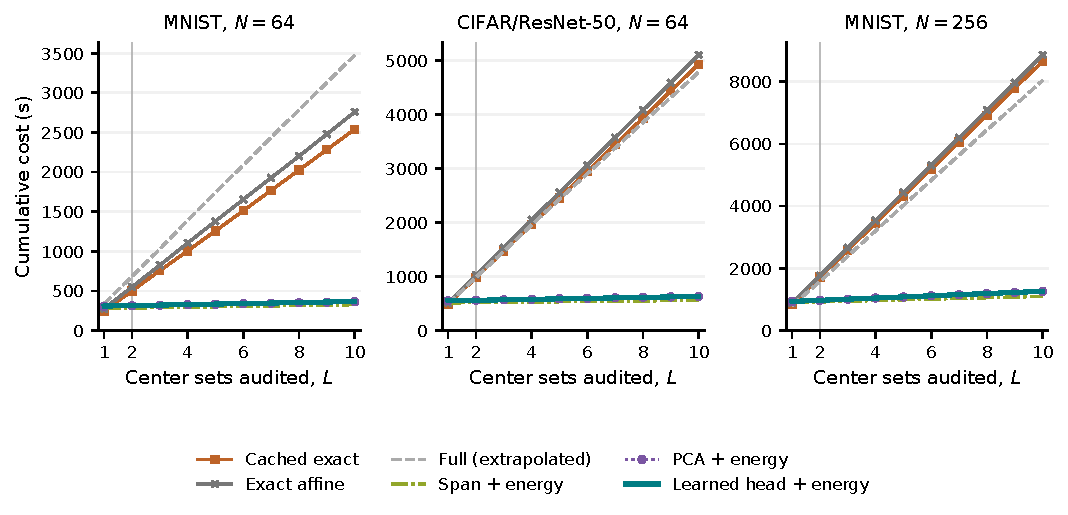
\includegraphics[width=\textwidth]{paper_results/reuse_revision/generated_20261020/cumulative_cost.pdf}
\caption{Cumulative cost for the three completed changing-center workloads. Learned head and PCA with energy almost overlap; savings over the tested center-specific cached/affine baselines come from reusing preprocessing and setup. The vertical line marks the second center set. Full catalog proving is extrapolated from one measured batch per set.}
\label{fig:reuse-cost}
\end{figure*}

For MNIST $N=64$, learned and PCA with energy have the same 519,896-constraint reuse circuit, compared with 343,455 for the narrower span-only head. Their Stage~1 circuits have 171,586 and 171,582 constraints per row. At $N=256$, the larger Merkle depth increases the shared reuse circuit to 568,022 constraints; learned Stage~1 uses 173,086 per row. For CIFAR, learned/PCA reuse requires 524,336 constraints and Stage~1 requires 432,049 per row. Selecting a different basis can therefore change accuracy without materially changing proof cost. Saved peak process-tree RSS is about 1.1--1.6\,GB for the 16-statistic methods; it excludes the Python driver and is not whole-pipeline memory.

\subsection{Changing-center fidelity}
The learned head has higher new-center agreement than PCA with energy on all three proof workloads: 98.26\% versus 96.53\% on MNIST $N=64$, 99.48\% versus 98.44\% on CIFAR embeddings, and 98.31\% versus 97.44\% on MNIST $N=256$ (Table~\ref{tab:reuse-quality}). The narrower deployed span alone reaches 83.51\%, 96.35\% and 85.76\%. Learned mean absolute cost errors are 0.228\%, 0.338\% and 0.178\%, compared with PCA/energy's 1.536\%, 0.441\% and 1.722\%. Cached and affine attain 100\% agreement, with small floating-reference cost differences due to quantization. Mean agreement is not a worst-case guarantee: learned agreement on the least accurate updated set is 95.31\%, 96.88\% and 94.92\%, respectively.
\begin{table*}[tp]
\caption{Answer fidelity on the nine new center sets in each proof workload.}\label{tab:reuse-quality}
\centering\small
\begin{adjustbox}{max width=\textwidth}
\begin{tabular}{@{}llrrr@{}}
\toprule
Catalog & Method & Mean agree. (\%) & Min. agree. (\%) & Mean $|e_\Psi|$ (\%) \\
\midrule
MNIST ($N=64$) & Cached exact & 100.00 & 100.00 & 0.003 \\
MNIST ($N=64$) & Exact affine & 100.00 & 100.00 & 0.003 \\
MNIST ($N=64$) & Span + energy & 83.51 & 67.19 & 1.977 \\
MNIST ($N=64$) & PCA + energy & 96.53 & 93.75 & 1.536 \\
MNIST ($N=64$) & Learned head + energy & 98.26 & 95.31 & 0.228 \\
CIFAR/ResNet-50 ($N=64$) & Cached exact & 100.00 & 100.00 & 0.002 \\
CIFAR/ResNet-50 ($N=64$) & Exact affine & 100.00 & 100.00 & 0.002 \\
CIFAR/ResNet-50 ($N=64$) & Span + energy & 96.35 & 89.06 & 0.757 \\
CIFAR/ResNet-50 ($N=64$) & PCA + energy & 98.44 & 96.88 & 0.441 \\
CIFAR/ResNet-50 ($N=64$) & Learned head + energy & 99.48 & 96.88 & 0.338 \\
MNIST ($N=256$) & Cached exact & 100.00 & 100.00 & 0.004 \\
MNIST ($N=256$) & Exact affine & 100.00 & 100.00 & 0.004 \\
MNIST ($N=256$) & Span + energy & 85.76 & 64.84 & 2.219 \\
MNIST ($N=256$) & PCA + energy & 97.44 & 95.31 & 1.722 \\
MNIST ($N=256$) & Learned head + energy & 98.31 & 94.92 & 0.178 \\
\bottomrule
\end{tabular}
\end{adjustbox}
\par\smallskip\begin{minipage}{0.98\textwidth}\footnotesize Agreement is against floating-point original-space Full on the same catalog rows. Means weight the nine new center sets equally; minimum is the worst set, not a confidence bound. Cached and affine are exact on quantized inputs, so their floating-reference cost errors can be nonzero.\end{minipage}
\end{table*}

This is an accuracy--reuse trade-off against exact recomputation and an accuracy comparison at similar proof cost against PCA. The nine updated sets reuse the same rows and fitted basis, so they are not nine independent dataset replications.

\subsection{Native new-center, shift and owner controls}
The broader native new-center grid evaluates budgets 16/32/64/128/256, two sparse-map densities and ten maps per randomized setting, subject to input dimension and PCA training-rank restrictions. It includes twelve new scenarios, adding changed center counts and another Lloyd snapshot to the proof workload's families. On matched cells, head+energy with a JL residual cross-term estimate is less accurate than PCA+energy at every tested budget. At budget 16 the agreement is 73.92\% versus 93.27\%; at 256 it is 91.16\% versus 98.13\% (Table~\ref{tab:reuse-jl}). The real same-center control gives 100\% agreement and maximum absolute relative cost error below $1.5\times10^{-15}$.
\begin{table*}[tp]
\caption{Native new-center comparison on matched cells: head/energy/JL versus PCA/energy.}\label{tab:reuse-jl}
\centering\small
\begin{adjustbox}{max width=\textwidth}
\begin{tabular}{@{}rrrrrr@{}}
\toprule
Budget & Cells & JL agree. (\%) & PCA/E agree. (\%) & JL $|e_\Psi|$ (\%) & PCA/E $|e_\Psi|$ (\%) \\
\midrule
16 & 720 & 73.92 & 93.27 & 5.852 & 0.673 \\
64 & 648 & 85.34 & 96.14 & 1.110 & 0.152 \\
256 & 504 & 91.16 & 98.13 & 0.326 & 0.037 \\
\bottomrule
\end{tabular}
\end{adjustbox}
\par\smallskip\begin{minipage}{0.98\textwidth}\footnotesize The tail estimates the residual cross term with one signed bucket per column. Maps are averaged within a corpus/$k$/start/scenario cell before aggregation. Eligibility differs across budgets; within each row both methods use identical cells. Native float64 computation, not proofs.\end{minipage}
\end{table*}


A follow-up tests learned-head/JL budget splits, $q=4,8$, SRHT maps, clipping and shrinkage. No tested hybrid improves the mean agreement over PCA with energy on its matched cells at any tested budget. The full learned head without a tail is also slightly below PCA/energy in this broader native comparison: 93.19\% versus 93.27\% agreement at budget 16, and 98.07\% versus 98.13\% at 256. Thus the learned method's higher agreement on the two proof catalogs does not extend to the aggregate native grid. The results motivate spending the residual budget on learned directions instead of a random cross-term estimator for the main circuit, while retaining PCA/energy as a strong baseline.

The shift/owner study comprises 60 jobs and 22,260 rows across five corpora. The owner simulation partitions training records among five owners with Dirichlet parameter 0.3; the residual/PCA basis sees only owner~0, while deployed public centers come from pooled training data. The shift simulation fits on old classes and tests new-only and mixed-class cases. At budget 16, learned head+energy reaches 89.89\% agreement versus 81.71\% for PCA/energy in the owner setting, but 74.50\% versus 76.33\% under shift. JL is weaker in both aggregate comparisons (Table~\ref{tab:reuse-shift}). These are native simulations with different information constraints, not federated proof or communication measurements.
\begin{table*}[tp]
\caption{Native budget-16 agreement under non-IID owners and class distribution shift.}\label{tab:reuse-shift}
\centering\small
\begin{adjustbox}{max width=\textwidth}
\begin{tabular}{@{}llrrr@{}}
\toprule
Setting & Method & Cells & Agree. (\%) & Matched PCA/E (\%) \\
\midrule
owners & Learned head + energy & 360 & 89.89 & 81.71 \\
shift & Learned head + energy & 60 & 74.50 & 76.33 \\
owners & Head/energy/JL ($q=4$) & 360 & 72.02 & 81.71 \\
shift & Head/energy/JL ($q=4$) & 60 & 60.14 & 76.33 \\
owners & Plain JL ($q=4$) & 360 & 55.38 & 81.71 \\
shift & Plain JL ($q=4$) & 60 & 58.48 & 76.33 \\
\bottomrule
\end{tabular}
\end{adjustbox}
\par\smallskip\begin{minipage}{0.98\textwidth}\footnotesize Five corpora, $k=5,10$, three starts. Random maps are averaged within each matched cell. Owners: residual/PCA fitting uses owner 0, while deployed public centers use pooled training rows. Shift: fit on old classes and audit new-only/mixed cases. These are native simulations.\end{minipage}
\end{table*}


\subsection{Binding and adaptive-map controls}
The existing circuit tests exercise honest in-span and out-of-span reuse, check that the in-span integer fixture agrees with Full, and reject altered costs, margins, assignments, authenticated heads and offsets. Earlier original-binding tests also cover missing Stage~1 indices, substituted roots and keys, and changed subset data. These are targeted engineering checks of the implemented relation.

The earlier native adaptive-map controls illustrate a different question (Table~\ref{tab:attack-controls}). With a known PCA map, the constructed perturbation changes about 97.6\% of assignments while leaving the projected claim unchanged. The corresponding fresh sparse-map control does not hide the same injected energy. These controls generate no forged end-to-end proofs and test a linear head/tail representation, not head+energy. They show why a faithfully executed known projection can be a poor proxy on adversarial data; the Stage~1 binding guarantee itself does not depend on a JL tail.
The detailed native perturbation table is retained in Appendix~\ref{app:attack}.

\section{Discussion}\label{sec:discussion}
\subsection{Choosing the representation}
For a single approved center set with repeated subset queries, cached exact answers are the strongest tested choice: the original-space integer argmin and cost are proved once and later authenticated cheaply. Affine scores retain all candidate fixed-center distances and are exact on the same integer inputs. Head and energy are useful when a common represented span supports several center sets, or when later approximate audits justify retaining more information than one cached answer.

The learned representation targets the latter use. Protecting the deployed span preserves its real-arithmetic comparisons, while residual PCA spends the remaining budget on training directions likely to matter for updates. The main proof workloads show a favorable combination of reuse cost and agreement, rather than a proof-speed advantage over equally reusable PCA with energy. The distribution-shift study further shows that learned head is not uniformly more accurate than PCA. Basis selection is an approximation policy that should be approved and evaluated for the intended queries.

The tested sparse-JL tails have a distinct reason to remain in the study: choosing a map without training data and analyzing its dependence on commitment order. Their negative fidelity results are evidence about the tested estimators and budgets. They neither invalidate JL theory nor establish that learned maps have a worst-case accuracy guarantee. Stage~1 binding applies to either approved map.

\subsection{Scope and limitations}
The completed changing-center proof evidence comprises two 64-record catalogs and one 256-record MNIST catalog, each with ten ordered center sets on one four-CPU Linux host. The larger MNIST catalog is a scale check on the same corpus and fitted-model configuration, not a third independent application. New-center sets are refits, subsamples, Lloyd snapshots and perturbations from a fixed training corpus. The completed eight-corpus five-start native campaign broadens fixed-center fidelity evidence, but does not substitute for larger-catalog, independent-model or cross-host proof replication.

Cumulative costs reconstruct sums of measured compilation, circuit-specific setup, native preparation, witness generation and median proving times. They are not observed wall-clock latency for an online deployment. They exclude public-model fitting, verification, warmups, I/O and new-center-statistic preparation. Full catalog proving is extrapolated from one actual batch per center set; cached, affine and reusable compressed methods prove all catalog rows and requested subsets. The crossover is relative to these concrete implementations, including center-specific setups for cached/affine and Full. A dynamic-center Full circuit or an in-span reusable affine parameterization would change the comparison.

All reuse methods prove an approximate original-space score outside the represented span, with exact execution only for their approved integer relation. The aggregate margin is not a per-record fidelity certificate. The study also excludes proof of model training, real federated communication, arbitrary-center worst-case guarantees, adaptive leakage bounds and full-corpus proof deployment. The benchmark verifies generated proofs inside the proving CLI. A fresh independent, public-only replay of the saved reuse bundles has not been completed; this artifact check should precede a public submission. A real model-update trace and larger catalogs would further test deployment relevance.

\section{Conclusion}\label{sec:conclusion}
Classical head coordinates and residual energy provide a compact interface for verifiable center-based audits. The system proves their derivation from committed original rows, then reuses the authenticated catalog across public center updates through one Stage~2 circuit. Across the completed 64-/256-row MNIST and 64-row CIFAR-embedding workloads, reuse beats the tested center-specific cached baseline from the second center set and reduces ten-set cumulative measured-component cost by factors of 6.82--7.76. The learned head achieves 98.26--99.48\% new-center agreement and improves on equally reusable PCA with energy on these proof catalogs at similar proof cost. The broader native evidence keeps that accuracy claim local to the tested catalogs. Exact cached and affine controls remain preferable for a single fixed task; sparse-JL tails remain a data-oblivious protocol option and an empirically weaker new-center baseline at the tested budgets.


\FloatBarrier
\onecolumn
\appendix
\numberwithin{table}{section}
\renewcommand{\thetable}{\Alph{section}.\arabic{table}}
\renewcommand{\theHtable}{appendix.\Alph{section}.\arabic{table}}
\renewcommand{\theHequation}{appendix.\Alph{section}.\arabic{equation}}
\section{Additional fixed-center evidence}\label{app:fixed}
The tables in this appendix retain the earlier completed Poseidon2 cohort and its native component/five-start follow-ups. They are not pooled with the new changing-center timing cohort. ``CommitJL'' in these retained tables means the protected head, energy and optional sparse tail; fixed-center assignment/cost queries do not use the tail. Native accuracy compares with quantized Full unless marked otherwise.
% Numerical contents retained from bound_revision; regular floats for the single-column appendix.
\begin{table}[!htbp]
\caption{Fixed-center fidelity on eight capped corpora at storage budget 16.}\label{tab:capped}
\centering\small
\begin{adjustbox}{max width=\textwidth}
\begin{tabular}{@{}lrrrrrr@{}}
\toprule
Corpus & $k$ & Sparse ARI & PCA ARI & Head/E ARI & PCA agree. (\%) & Head/E agree. (\%) \\
\midrule
Gaussian-easy & 5 & 0.62947 & 1.00000 & 1.00000 & 100.000 & 100.000 \\
Gaussian-easy & 10 & 0.87790 & 1.00000 & 1.00000 & 100.000 & 100.000 \\
Gaussian-hard & 5 & 0.11602 & 0.99365 & 1.00000 & 99.792 & 100.000 \\
Gaussian-hard & 10 & 0.15151 & 0.99359 & 1.00000 & 99.000 & 100.000 \\
Margin-synthetic & 5 & 0.18329 & 0.62386 & 0.99640 & 89.833 & 99.917 \\
Margin-synthetic & 10 & 0.21543 & 0.49844 & 1.00000 & 79.167 & 100.000 \\
MNIST & 5 & 0.36872 & 0.98165 & 0.99960 & 99.183 & 99.983 \\
MNIST & 10 & 0.36090 & 0.92547 & 0.99964 & 96.567 & 99.983 \\
Fashion-MNIST & 5 & 0.66488 & 0.99484 & 1.00000 & 99.783 & 100.000 \\
Fashion-MNIST & 10 & 0.64867 & 0.98679 & 0.99958 & 99.317 & 99.983 \\
Gisette & 5 & 0.14792 & 0.96671 & 0.99917 & 98.694 & 99.972 \\
Gisette & 10 & 0.12200 & 0.92786 & 1.00000 & 96.861 & 100.000 \\
Arcene & 5 & 0.85164 & 1.00000 & 1.00000 & 100.000 & 100.000 \\
Arcene & 10 & 0.67673 & 0.95751 & 1.00000 & 97.500 & 100.000 \\
20 Newsgroups & 5 & 0.01789 & 0.82891 & 1.00000 & 93.511 & 100.000 \\
20 Newsgroups & 10 & 0.00868 & 0.61244 & 1.00000 & 78.988 & 100.000 \\
\bottomrule
\end{tabular}
\end{adjustbox}
\par\vspace{3pt}\begin{minipage}{0.98\textwidth}\footnotesize Reference: quantized Full. Means over three fitted starts; sparse maps are averaged within a start before aggregation. Head/E and CommitJL have identical fixed-center outputs. Sparse JL uses one signed bucket per input column. ARI measures assignment fidelity, not agreement with class labels.\end{minipage}
\end{table}

\begin{table}[!htbp]
\caption{Actual whole-catalog query on 64 committed MNIST records, $k=5$.}\label{tab:query64}
\centering\small
\begin{adjustbox}{max width=\textwidth}
\begin{tabular}{@{}lrr@{}}
\toprule
Method & Constraints & Proving time (s) \\
\midrule
PCA-16 & 472,429 & 6.303 \\
Head + energy & 306,275 & 5.341 \\
CommitJL-16 & 306,274 & 5.087 \\
Exact affine & 271,205 & 5.240 \\
Cached exact & 197,147 & 3.442 \\
\bottomrule
\end{tabular}
\end{adjustbox}
\par\vspace{3pt}\begin{minipage}{0.98\textwidth}\footnotesize Same original catalog and centers for all methods; each saved proof independently verifies. This is one possible 64-record subset, with three timing repetitions after warmup. Full was measured only at $q=1$ for this catalog; no large-shape Full estimate is inserted. The one-constraint head/E difference comes from compiled context details, not useful tail computation.\end{minipage}
\end{table}

\begin{table}[!htbp]
\caption{Preprocessing and reconstructed fresh-workload cost, MNIST $N=64$, $k=5$.}\label{tab:preprocessing}
\centering\small
\begin{adjustbox}{max width=\textwidth}
\begin{tabular}{@{}lrrrrr@{}}
\toprule
Method & \shortstack{Stage-1\\constraints/row} & \shortstack{Median row\\proof (s)} & \shortstack{All row\\proofs (s)} & \shortstack{Stage-1\\compile/setup (s)} & \shortstack{Four-query\\workload (s)} \\
\midrule
PCA-16 & 170,744 & 3.087 & 197.961 & 29.011 & 279.123 \\
Head + energy & 168,901 & 3.067 & 196.990 & 28.372 & 264.617 \\
CommitJL-16 & 174,208 & 3.083 & 198.221 & 29.350 & 268.383 \\
Exact affine & 168,815 & 3.058 & 195.780 & 29.559 & 268.288 \\
Cached exact & 168,446 & 3.014 & 194.488 & 27.153 & 246.660 \\
\bottomrule
\end{tabular}
\end{adjustbox}
\par\vspace{3pt}\begin{minipage}{0.98\textwidth}\footnotesize The workload uses four genuinely distinct 32-record subsets. It adds native Go preparation, all 64 Stage-1 witness/proof costs, Stage-1 and query compilation/setup, and one witness/proof per subset. Public-model fitting, verification, warmups and I/O are excluded. These sums reconstruct measured components; they are not observed elapsed times or an empirical break-even threshold.\end{minipage}
\end{table}


\FloatBarrier

\Needspace{10\baselineskip}
\section{Native perturbation control}\label{app:attack}
This earlier control tests whether a native linear head/tail projection can conceal injected energy when its map is known. It does not construct a forged proof and does not attack the head+energy relation. The output definitions and limitations are retained with the original numerical values.
\begin{table}[!htbp]
\caption{Earlier native perturbation controls; no forged end-to-end proofs are generated.}\label{tab:attack-controls}
\centering\scriptsize
\begin{adjustbox}{max width=\textwidth}
\begin{tabular}{@{}lllll@{}}
\toprule
Projection/order & True inflation & Claim inflation & Flip fraction & Honest error \\
\midrule
pca\_public & 11.000 & 1.000 & 0.9762 & 0.0273 \\
protected\_commit & 11.000 & 11.010 & 0.0000 & 0.0000 \\
protected\_prepublished & 11.000 & 1.000 & 0.0000 & 0.0000 \\
sparse\_commit & 10.988 & 11.138 & 0.6082 & 0.3715 \\
sparse\_prepublished & 10.988 & 1.000 & 0.8578 & 0.3713 \\
\bottomrule
\end{tabular}
\end{adjustbox}
\par\smallskip
\begin{minipage}{\textwidth}\scriptsize Protected rows test the linear head+tail representation, not head+energy. Fresh-map rows use one independently guessed-map strategy. Flip and honest-error fractions concern different point sets and cannot be subtracted to isolate attack advantage. The unverified internal Pisot surrogate is excluded from comparisons with published methods.\end{minipage}
\end{table}

\FloatBarrier

\section{Data-oblivious sparse-map specification}\label{app:jl}
The canonical generator uses domain-separated SHAKE-256 streams for bucket indices and signs. For each original coordinate it draws $q$ distinct bucket indices by rejection and independent signs, retaining a canonical ordered encoding. Reducing a fixed-width word modulo $m$ without rejecting the biased prefix is not uniform; \path{code/commitjl/sparse_gen.py} implements the canonical rejection specification. Generator expansion and challenge approval are verifier-side checks, rather than an in-circuit XOF proof in the measured reuse system.

Under ideal independent zero-mean signs and the specified column sampling, $\mathbb E[\|Av\|^2/q]=\|v\|^2$: expand the square, cancel cross terms by sign independence, and count the $q$ diagonal contributions per coordinate. This is a first-moment statement, not a concentration bound. A tail estimator for the missing inner product uses $\langle Ar(x),Ar(c')\rangle/q$ in Eq.~\eqref{eq:new-center-exact}; its noise explains why adding a tail need not improve assignment fidelity at a fixed storage budget.

For commitment order, eligible roots and a digest of the relevant centers/task are registered before a fresh challenge. A verifier nonce, a beacon round with a registration deadline, or a commit--reveal protocol can supply the entropy. A task log must bound eligible attempts when claiming a task-level geometric failure probability. Root-derived deterministic randomness alone permits offline search over commitment salts. Public reproducibility is not sufficient to establish independence from adversarially chosen inputs.

\section{Quantization and evidence provenance}\label{app:configurations}
With per-coordinate rounding error at most $1/(2S)$, each point has Euclidean error at most $\sqrt d/(2S)$. For two points $u,v$, write the difference error as $\eta$, where $\|\eta\|\le\sqrt d/S$. Expanding $\|(u-v)+\eta\|^2$ gives the additive bound
\begin{equation}
\begin{aligned}
&\left|\|\widetilde u/S-\widetilde v/S\|^2-\|u-v\|^2\right|\\
&\qquad\le2\|u-v\|\sqrt d/S+d/S^2.
\end{aligned}
\end{equation}
Rounded-basis error and the omitted new-center cross term are separate from this input perturbation. The integer row bounds in Eq.~\eqref{eq:row-bounds} do not assert an original-space approximation ratio.

The current export manifest is \path{paper_results/reuse_revision/generated_20261020/manifest.json}; it records input hashes, exact cumulative costs, crossover calculations and five-start cell coverage. The completed snapshot observed at 20:32 UTC on 19 October 2026 (00:02 Tehran time on 20 October) contains both $N=64$ workloads, the complete $N=256$ workload and all three native fidelity workers. Its analysis checks 1,092 captured hashes and reconstructs exported proof costs from the saved phase samples. The fidelity export contains all 80 expected corpus/$k$/start cells with no duplicate non-ablation method/width/map rows. The legacy head-only ablation is emitted once per eligible width; those repeated entries are excluded from the width-16 comparison. Earlier fixed-center exports retain their own manifests under \path{paper_results/bound_revision}. Full raw arrays and saved proof artifacts remain in preserved experiment folders; the source package includes numerical exports and provenance rather than all proving artifacts.

\FloatBarrier
\twocolumn
\section*{Declarations}
\paragraph{Author information, contributions and acknowledgements}
Names, affiliations, corresponding-author details, contributor roles and acknowledgements require author confirmation before submission.
\paragraph{Funding and competing interests}
Funding sources and the competing-interest declaration require confirmation by all authors.
\paragraph{Data and code availability}
The experiments use the public benchmark sources cited in Table~\ref{tab:datasets-a} and synthetic data. The research artifact preserves loaders, circuit and analysis code, configuration records, captured output hashes and raw benchmark results. A public repository or persistent archive identifier has not yet been assigned. The portable paper source package includes the numerical exports and their provenance; large datasets and proof bundles remain separate.
\paragraph{Ethics and consent}
The final ethics and consent declarations require author review of the benchmark data sources and intended release. No claim of new collection of sensitive participant records is made in this study.
\paragraph{Declaration of generative AI and AI-assisted technologies in the manuscript preparation process}
OpenAI Codex assisted with source-code development, result aggregation, literature navigation, manuscript organization and language revision. Numerical claims are derived from retained experiment outputs and deterministic analysis scripts. The human authors are responsible for checking the code, sources, interpretation and complete manuscript, and for approving the final submission. AI tools are not authors.

\bibliographystyle{elsarticle-num}
\bibliography{references}
\end{document}
